
The controller system’s architecture has been modelled such that the safety and liveness requirements are always met, by using the various sensors, actuators, and other components that are present in the system.

The main assumptions made here for simplicity are as follows. The robots perform the instructed actions without any error. The lamp performs the projecting process without malfunctioning. The other components may require the user to act upon them based on certain sensor data and the corresponding user inputs described as interactions in chapter~{\ref{chap:interact}}.

\begin{figure}[h]
\centering
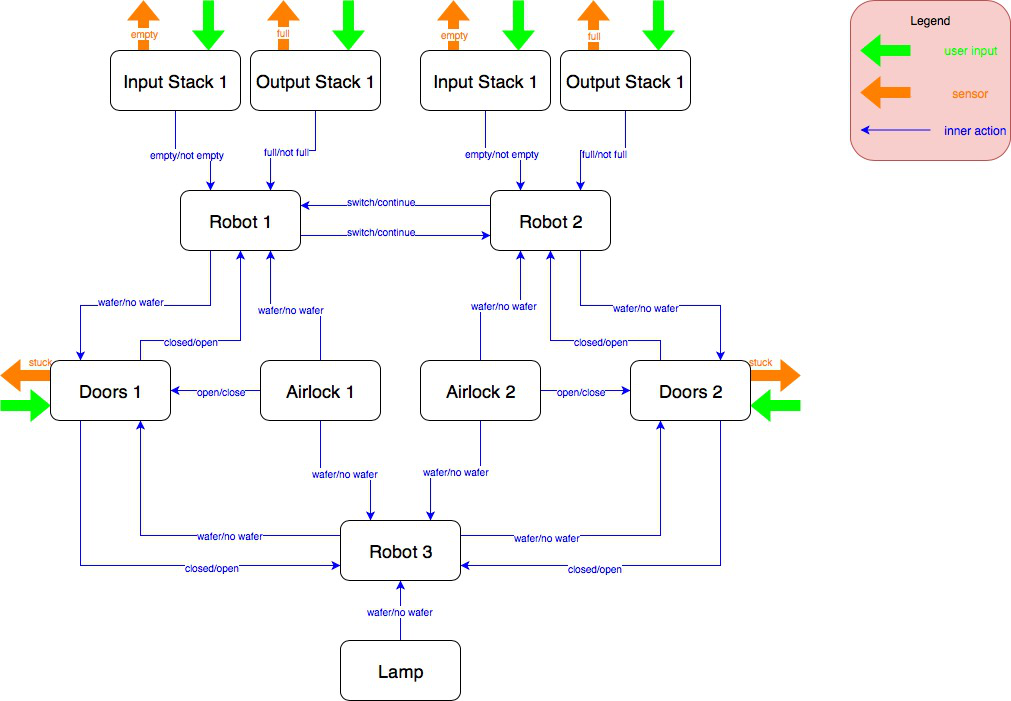
\includegraphics[width=150mm]{img/sv-project-arch.png}
\caption{System architecture diagram\label{fig:arch}}
\end{figure}

The architecture of the system is represented graphically using the Figure~{\ref{fig:arch}}. It consists of several components working in parallel to meet the requirements stated in chapter~{\ref{chap:reqs}}.

For the most part, the system is expected to function without the need for any user input, but certain cases have been identified in which user input is needed to meet the system’s liveness requirements. These are indicated by green arrows in the diagram, and the corresponding sensor action indicating the need for user input is shown using orange arrows.

The system never reaches a state of “completion” since it is expected to run continuously till one of the conditions requiring a user input is met (see chapter~{\ref{chap:reqs}}). Theoretically, if the user continually
replenishes the input stack with new wafers and clears the output stack at the same rate, and if the airlock doors do not malfunction, the system can run for an indefinite period of time.
